

%%%%%%%%%%%%%%%%%%%%%%%%%%%%%%%%%%
% Cells
%%%%%%%%%%%%%%%%%%%%%%%%%%%%%%%%%%
\section{Cells}
\par The cell is the basic unit of life. At the fundamental level, a cell must have an outer membrane that acts as a gatekeeper between the surrounding environment and the interior constituents. The actual contents of the cell interior vary widely between between the classes of prokaryotes (single-celled organisms) and eukaryotes (cells of multi-celled organisms), and even between different instances of the classes and different states of those instances. For example, mature red blood cells do not contain a nuclei or any genetic material, but skeletal muscle fiber consist multiple nuclei. However, all these variations can be generalized to useful cell models, such as the model for human cells in figure \ref{fig:human_cell_model}.   
\begin{figure}[ht]
 \centering
 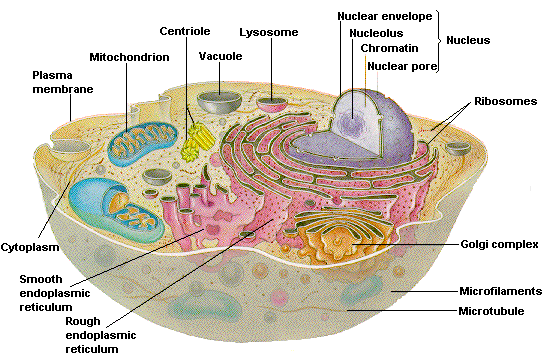
\includegraphics[width=0.7\textwidth]{images/humanCellOverview.png}
 \caption[Diagram of human cell structure.]{Diagram of human cell structure. \cite{daniel_d_chiras_human_2005} }
 \label{fig:human_cell_model}
 \end{figure}
 
 
 \par Generally, a cell carries genetic information in the nucleus inside the cell membrance and cytoplasm. Cytoplasm is all cell material inside of the cell membrane except the nuclei. The cytoplasm consists of non-nuclei organelles and cytosol.  Cytosol refers to the cellular solution between the cell organelles and the membrane, wich contains salts, nucleic acids and cytoskeleton filaments. Organnelles are membrane bound structures inside the cell that perform a special function. Organelles include nuclei, mitochondria, the Golgi apparatus, lysosomes, and vacuoles.  
 
 \par All of these 
 
 %%%%%%%%%%%%%%%%%%%%%%%%%%%%%
 % The Cell Membrane
 %%%%%%%%%%%%%%%%%%%%%%%%%%%%%
 \subsection{The Cell Membrane}
 
 
 %%%%%%%%%%%%%%%%%%%%%%%%%%%%%%%%%%%%%%%%%
 % Electrical Model of the Cell
 %%%%%%%%%%%%%%%%%%%%%%%%%%%%%%%%%%%%%%%%%
 \subsection{Electrical Model of the Cell}
 
 
 %%%%%%%%%%%%%%%%%%%%%%%%%%%%%%%%
 % Dielectric Spectroscopy
 %%%%%%%%%%%%%%%%%%%%%%%%%%%%%%%%
 \section{Dielectric Spectroscopy}
 
 % Read into articles and provide more details
 
 \par The dielectric properties of cell have been investigated since 1910 when H\"{o}ber showed the existence of the cell membrane by measuring the conductivity of erythrocytes (red blood cells) at high and low frequencies \cite{hober_r_methode_1910}. The field of study further developed with Fricke's application of Maxwell's equations to measure the capacitance and thickness of the cell membrane in 1924-1925 \cite{james_clerk_maxwell_treatise_1892, fricke_h_mathematical_1924, fricke_h_electric_1924, fricke_h_electric_1931}. 
 
 \par Then in 1998, Cole used Maxwell's mixture equation to derive the complex impedance of a single shelled cell model and developed equations to describe the Cole-Cole plot \cite{cole_electric_1928}. And with Curtis, Cole made the first singel cell measurements on a Nitella cell \cite{curtis_transverse_1937}. A Nitella cell is a large bacteria cell that ranges in length from 20 $\mu$m to 60 mm. 
 
 \par From 1957-1968 Schwan used broadband electric impedance spectroscopy to identify $\alpha$, $\beta$, and $\gamma$ dispersions of a cell \cite{schwan_h_p_electrical_1957,schwan_h_p_electrical_1963,schwan_electrical_1994}. Where a dielectric dispersion is a relationship between an applied electric field and the permittivity of a material. The permittivity is the resistance to forming an electric field over a medium, and can be defined as
 
 \begin{equation}
     \textbf{D} = \epsilon \textbf{E}
 \end{equation}
 
 \noindent Where $\textbf{D}$ is the electric displacement tensor and represents how the electric field affects the organization of charges in a medium, $\epsilon$ is the permittivity, and $\textbf{E}$ is the electric field tensor. The $\alpha$, $\beta$, and $\gamma$ dispersions refers to the dielectric relaxation or ranges of alternating current frequencies where the permittivity decreases significantly. Figure \ref{fig:schwan_dispersions} depicts an approximate permittivity spectrum of a cell.
 
 \begin{figure}[ht]
 \centering
 
\includegraphics[width=0.7\textwidth]{images/schwanDispersions.png}
 \caption[General cell permittivity spectrum]{General cell permittivity spectrum with labeled $\alpha$, $\beta$ and $\gamma$ dispersions.}
 \label{fig:schwan_dispersions}
 \end{figure}
 
 \noindent $\beta$ dispersion occurs up to 10 Mhz and is caused by the relaxation of the cell membrane. For lower frequencies, the membrane has enough time to charge and provide resistance to the electric field, but at frequencies greater than ~10 Mhz, the membrane does not have sufficient time to fully charge and provides little resistance to the electric field. $\gamma$ dispersion is related to the relaxation of water molecules. Instead of a charging membrane, $\gamma$ dispersion is due to the dipole rotation of the of water molecules and the biomolecule that water is bound to. The source of $\alpha$ dispersion is undetermined, but current theories include the surface reactance of the electric double layer near the charged cell, the impedance of the sarcoplasmic recticulum (only for muscle fibers), or the frequency dependent conductance of ionic membrane channels as predicted by the Hodgkin-Huxley equations \cite{schwan_electrical_1994}.
 
 
 \par These developments laid the foundations for the following techniques for measuring the dielectric properties of single cells. 
 
 %%%%%%%%%%%%%%%%%%%%%%%%%%%%%%%%
 % Dielectrophoresis
 %%%%%%%%%%%%%%%%%%%%%%%%%%%%%%%%
 \subsection{Dielectrophoresis}
 \par The dielectrophoretic force (DEP) is the force generated on a particle suspended in a solution by the interaction of the applied nonuniform electric field and the induced dipole moment. Peter Debye and Herbert A. Pohl were among the first to develop dielectrophoresis and demnostrated how particles could be moved with nonuniform electric fields \cite{muller_potential_2003}. With an applied ac electric field, the average DEP force is expressed by \cite{morgan_single_2007, green_dielectrophoresis_1999}
 
 \begin{equation}
     \big< F_{DEP} \big> = \pi \epsilon_m R^3 \text{Re}[\tilde{f}_{CM}] \nabla |\textbf{E}|^2 \;\;\; \text{with} \;\;  \tilde{f}_{CM} = \frac{\tilde{\epsilon}_p - \tilde{\epsilon}_m}{\tilde{\epsilon}_p + 2\tilde{\epsilon}_m} 
 \end{equation}
 
 \noindent where $\epsilon_m$ is the permittivity of the medium, $R$ is the radius of the particle, $\tilde{f}_{CM}$ is the Clausius-Mossotti factor,  $\tilde{\epsilon}_p$ is the complex permittivity of the particle, $\tilde{\epsilon}_m$ is the complex permittivity of the medium, and $\textbf{E}$ is the electric field. For most cases, the complex permittivity can be expressed as 
 
 \begin{equation}
     \tilde{\epsilon} = \epsilon - j\frac{\sigma}{\omega}
 \end{equation}
 
\noindent where $\epsilon$ is the permittivity, $j = \sqrt{-1}$, $\sigma$ is the conductivity, and $\omega$ is the angular frequency. 
 
 %%%%%%%%%%%%%%%%%%%%%%%%%%%%
 % Electrorotation
 %%%%%%%%%%%%%%%%%%%%%%%%%%%%
 \subsection{Electrorotation}
 
 
 % However, a major shortcoming of the previously discussed techniques is long time for measurements. An electrorotaion assay could potentially take up to several seconds per test and, as a result, limit the number of cells tested
 
 %%%%%%%%%%%%%%%%%%%%%%%%%%%%%%%%%%%%%%%%%%%%%
 % Electrical Impedance Spectroscopy
 %%%%%%%%%%%%%%%%%%%%%%%%%%%%%%%%%%%%%%%%%%%%%
 \subsection{Electrical Impedance Spectroscopy}
 
 
 % Electrical impedance spectroscopy has historically only been used on multiple cells to obtain aggregate data, however, with the rise of microelectomechanical systems (MEMS) and microfluidics, electrical impedance spectroscopy can be applied to individualy cells.
 
 
 %%%%%%%%%%%%%%%%%%%%%%%%%%%%%%%%%%%%%%%%%%%%%%%%%%%%%%%%%
 % Microelectromechanical Systems and Microfluidics
 %%%%%%%%%%%%%%%%%%%%%%%%%%%%%%%%%%%%%%%%%%%%%%%%%%%%%%%%%
 \section{Microelctromechanical Systems and Microfluidics}
 
 %%%%%%%%%%%%%%%%%%%
 % MEMS
 %%%%%%%%%%%%%%%%%%%
 \subsection{MEMS}
 
 
 %%%%%%%%%%%%%%%%%%%%%%%%%%
 % Microfluidics
 %%%%%%%%%%%%%%%%%%%%%%%%%%
 \subsection{Microfluidics}
 
 
 %%%%%%%%%%%%%%%%%%%%%%%%%%%%%%%%%%%%%%%%%%%%%%%%%%%%%%%%%%%%%%%%%%%
 % Previous Work on the Cal Poly Biofluidic Lab's EIS System
 %%%%%%%%%%%%%%%%%%%%%%%%%%%%%%%%%%%%%%%%%%%%%%%%%%%%%%%%%%%%%%%%%%%
 \section{Previous Work on the Cal Poly Biofluidic Lab's EIS System}
 
 % In 2009 Josh Fadriuela and Stephanie Hernandez fulfilled their thesis under Dr.Clague to create a cell impedance sensor system. Their work will be the foundation for this thesis \cite{fadriquela_design_2009-1}, \cite{hernandez_single_2009-1}.
 